\documentclass[11pt]{article}

%% MinionPro fonts 
%\usepackage[lf]{MinionPro}
%\usepackage{MnSymbol}
\usepackage{microtype}

%% Margins
\usepackage{geometry}
\geometry{verbose,letterpaper,tmargin=1in,bmargin=1in,lmargin=1in,rmargin=1in}

%% Other packages
\usepackage{amsmath}
\usepackage{amsthm}
\usepackage[shortlabels]{enumitem}
\usepackage{titlesec}
\usepackage{soul}
\usepackage{tikz}
\usepackage{mathtools}
\usepackage{pgfplots}
\usepackage{tikz-3dplot}
\usepackage{algorithmic}
\usepackage[export]{adjustbox}
\usepackage{tcolorbox}
\usepackage{mathrsfs}

%% Paragraph style settings
\setlength{\parskip}{\medskipamount}
\setlength{\parindent}{0pt}

%% Change itemize bullets
\renewcommand{\labelitemi}{$\bullet$}
\renewcommand{\labelitemii}{$\circ$}
\renewcommand{\labelitemiii}{$\diamond$}
\renewcommand{\labelitemiv}{$\cdot$}

%% Colors
\definecolor{rred}{RGB}{204,0,0}
\definecolor{ggreen}{RGB}{0,145,0}
\definecolor{yyellow}{RGB}{255,185,0}
\definecolor{bblue}{rgb}{0.2,0.2,0.7}
\definecolor{ggray}{RGB}{190,190,190}
\definecolor{ppurple}{RGB}{160,32,240}
\definecolor{oorange}{RGB}{255,165,0}

%% Shrink section fonts
\titleformat*{\section}{\normalsize\bf}
\titleformat*{\subsection}{\normalsize\bf}
\titleformat*{\subsubsection}{\normalsize\it}

% %% Compress the spacing around section titles
\titlespacing*{\section}{0pt}{1.5ex}{0.75ex}
\titlespacing*{\subsection}{0pt}{1ex}{0.5ex}
\titlespacing*{\subsubsection}{0pt}{1ex}{0.5ex}

%% amsthm settings
\theoremstyle{definition}
\newtheorem{problem}{Problem}
\newtheorem{example}{Example}
\newtheorem*{theorem}{Theorem}
\newtheorem*{bigthm}{Big Theorem}
\newtheorem*{biggerthm}{Bigger Theorem}
\newtheorem*{bigcor1}{Big Corollary 1}
\newtheorem*{bigcor2}{Big Corollary 2}

%% tikz settings
\usetikzlibrary{calc}
\usetikzlibrary{patterns}
\usetikzlibrary{decorations}
\usepgfplotslibrary{polar}

%% algorithmic setup
\algsetup{linenodelimiter=}
\renewcommand{\algorithmiccomment}[1]{\quad// #1}
\renewcommand{\algorithmicrequire}{\emph{Input:}}
\renewcommand{\algorithmicensure}{\emph{Output:}}

%% Answer box macros
%% \answerbox{alignment}{width}{height}
\newcommand{\answerbox}[3]{%
  \fbox{%
    \begin{minipage}[#1]{#2}
      \hfill\vspace{#3}
    \end{minipage}
  }
}

%% \answerboxfull{alignment}{height}
\newcommand{\answerboxfull}[2]{%
  \answerbox{#1}{6.38in}{#2} 
}

%% \answerboxone{alignment}{height} -- for first-level bullet
\newcommand{\answerboxone}[2]{%
  \answerbox{#1}{6.0in}{#2} 
}

%% \answerboxtwo{alignment}{height} -- for second-level bullet
\newcommand{\answerboxtwo}[2]{%
  \answerbox{#1}{5.8in}{#2}
}

%% special boxes
\newcommand{\wordbox}{\answerbox{c}{1.2in}{.7cm}}
\newcommand{\catbox}{\answerbox{c}{.5in}{.7cm}}
\newcommand{\letterbox}{\answerbox{c}{.7cm}{.7cm}}

%% Miscellaneous macros
\newcommand{\tstack}[1]{\begin{multlined}[t] #1 \end{multlined}}
\newcommand{\cstack}[1]{\begin{multlined}[c] #1 \end{multlined}}
\newcommand{\ccite}[1]{\only<presentation>{{\scriptsize\color{gray} #1}}\only<article>{{\small [#1]}}}
\newcommand{\grad}{\nabla}
\newcommand{\ra}{\ensuremath{\rightarrow}~}
\newcommand{\maximize}{\text{maximize}}
\newcommand{\minimize}{\text{minimize}}
\newcommand{\subjectto}{\text{subject to}}
\newcommand{\trans}{\mathsf{T}}
\newcommand{\bb}{\mathbf{b}}
\newcommand{\bx}{\mathbf{x}}
\newcommand{\bc}{\mathbf{c}}
\newcommand{\bd}{\mathbf{d}}

%% LP format
%    \begin{align*}
%      \maximize \quad & \mathbf{c}^{\trans} \mathbf{x}\\
%      \subjectto \quad & A \mathbf{x} = \mathbf{b}\\
%                       & \mathbf{x} \ge \mathbf{0}
%    \end{align*}


%% Redefine maketitle
\makeatletter
\renewcommand{\maketitle}{
  \noindent SA405 -- AMP \hfill Rader \S 3.4 \\

  \begin{center}\Large{\textbf{\@title}}\end{center}
}
\makeatother

%% ----- Begin document ----- %%
\begin{document}
  
\title{Lesson 10,  Combinatorial Models:  Minimum Spanning Tree}

\maketitle

%%%

\section{Combinatorial Models}

Many optimization problems are naturally modeled by a combinatorial structure, such as a \textbf{graph}. For the next few weeks, we will be talking about several famous combinatorial optimziation problems: \emph{minimum spanning tree}, \emph{traveling salesperson}, and \emph{vehicle routing problem}. 

Combinatorial optimization problems are usually more general than the network problems we've seen before as they operate on a \textbf{graph} instead of a \textbf{network}. Recall that a network is a special type of graph.

%\textbf{Usually the best solution strategies for combinatorial problems are algorithms or heuristics that explicitly leverage the graphical structure of the problem.}  We will see examples of such strategies later in the course.
%
For now, we will develop integer programs to model these problems. Integer programming is appropriate for traveling salesperson and vehicle routing problems (they're NP-Complete which means \textbf{really} hard to solve); but, like the other networks we have done so far, there are more efficient ways to handle MST.
%
%What is the difference between an \textbf{algorithm} and a \textbf{heuristic}?
%
%\answerboxfull{c}{2in}
%
%Is the simplex method an algorithm or a heuristic?
%
%\answerboxfull{c}{1in}


\section{Graph Terminology}


Suppose $G = (V,E)$ is an \emph{undirected} graph. (So far we have worked with directed graphs.) Recall that:
	\begin{itemize}
	\item $V$ is the set of vertices or nodes
	\item $E$ is the set of edges
	\end{itemize}

An undirected graph is different in that the edges can now be traversed in both directions. \vspace{1in}

As a result, it's good to be consistent in naming the edges. For example, using our old style of naming, an edge connecting nodes 1 and 2 could be both $x_{1,2}$ and $x_{2,1}$. As a result, we will always name edges from lower index to higher index.

\newpage


\begin{tcolorbox}
Graph $G$ is \textbf{connected} if for \emph{every} pair of vertices $a,~b \in V$, there exists a \textbf{path} of edges in $G$ connecting $a$ and $b$.  
\end{tcolorbox}

Example: \vspace{2in}

\begin{tcolorbox}
A \textbf{cycle} is a closed path of nodes meaning that the first and last node in the path is the same vertex.
\end{tcolorbox}

Example: \vspace{2in}

\begin{tcolorbox}
If $G$ is a connected graph that contains a \textbf{cycle}, then the removal of a single edge from the cycle does not destroy the connectivity of $G$.
\end{tcolorbox}

\begin{enumerate}[resume]
\item Illustrate a cycle and prove the fact that if $G$ has a cycle, removing any edge from the cycle does not make the graph disconnected.
\end{enumerate}

\newpage



\begin{tcolorbox}
A connected graph that contains no cycles is called a \textbf{tree}.  
\end{tcolorbox} \vspace{3in}

\begin{tcolorbox}
Trees are \textbf{minimally connected}:  if we remove any edge from a tree, the resulting graph is disconnected.
\end{tcolorbox}
\begin{enumerate}[resume]
\item Convince yourself of the previous fact by drawing a tree on 6 vertices.  Are there any edges you can remove from the graph without losing connectivity?
\end{enumerate}

\vfill

Side note: Trees are really important in tons of real world problems. For example, every time you make a Google search or use GoogleMaps an algorithm is called where one of the key parts is analyzing a huge tree. \vspace{1cm}


\newpage
\begin{tcolorbox}
A \textbf{spanning tree} of a graph $G$ is a  subset of the edges of $G$ that form a 
\emph{tree that connectes every vertex in $V$} (i.e., it spans the nodes of $G$).
\end{tcolorbox}


\begin{enumerate}[resume]
\item Consider the graph $G$ on 5 vertices below.  

\begin{center}
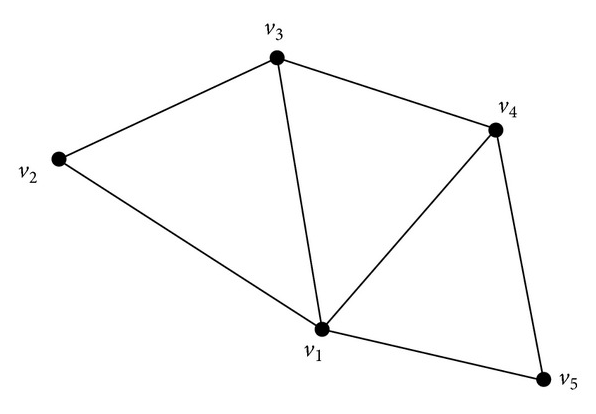
\includegraphics[width=.4\textwidth]{graph5}
\end{center}

\begin{itemize}
\item[(a)] Draw two different spanning trees of $G$.

\vspace{2.5in}

\item[(b)] How many edges does each spanning tree have?  \letterbox
\item[(c)] List the elements (edges) of the spanning tree. 

\vspace{1in}
\item[(d)] How many edges does a spanning tree of a graph $G$ with vertex set $V$ have in general?

\end{itemize}
\end{enumerate}

\newpage
\section{Minimum Spanning Tree (MST) Problem}

\begin{tcolorbox}
Associate a cost $c_{ij}$ with every edge $(i,j) \in E$. The problem of finding the \emph{spanning tree} of graph $G$ with \emph{minimum edge cost} is known as the \textbf{minimum spanning tree problem}.
\end{tcolorbox}

\begin{itemize}
\item  Real world applications of the minimum spanning tree problem include planning road, electrical, data, phone, and water networks.  
\end{itemize}

\bigskip

\begin{enumerate}[resume]
\item  Solve the minimum cost spanning tree problem for the graph shown below.  (The numbers on the edges are the edge costs.)

\begin{center}
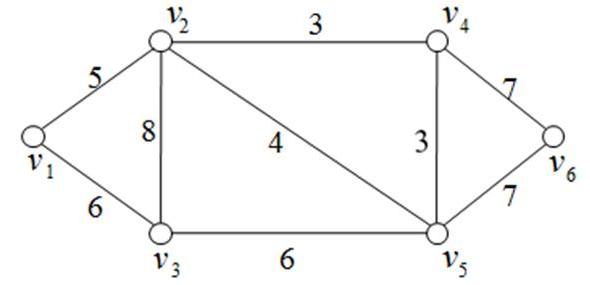
\includegraphics[width = 0.7\textwidth]{weightedgraph}
\end{center}

Minimum spanning tree $T =$ 


\end{enumerate}


\newpage
\section{MST IP Formulation}
\emph{It is more efficient to solve a min-cost spanning tree problem via an algorithm (like maybe from SA403), it is still instructive to model it using IP. Specifically because fully understanding the MST problem formulation will be helpful in understanding traveling salesperson and vehicle routing.}

A local phone company is interested in laying cable from the main road (where the
Main switch is located) to a new housing subdivision, and wants to do so in the least
expensive way.  It has the option of laying cable from the road to any house, or it can 
lay cable between the houses.  Each house must be connected through some path to 
the road.  The following matrix gives the total cost of laying cable between any two
locations, where the first location is the main road.

\begin{center}
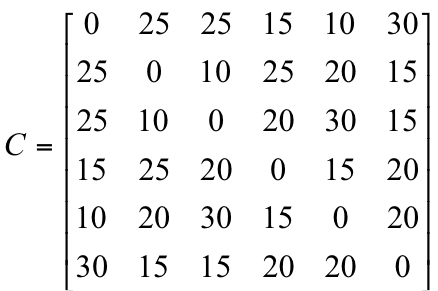
\includegraphics[width = .3\textwidth]{costs}
\end{center}

How should the phone company connect the houses to the road in order to minimize its
total cost?

\begin{enumerate}[resume]
\item Draw a graph to represent this problem below. 

\vfill

\item Define the \textbf{sets}, \textbf{variables}, and \textbf{parameters} for the problem.  
\vfill 
\newpage

\item Write the objective function in both concrete and parameterized form. \vspace{1.5in}

\item Minimum spanning trees must touch every vertex.  Write a concrete constraint that ensures that vertex 1 is covered by the spanning tree returned by the solver.  Do the same for vertices 2 and 3.  Finally, write an parameterized class of constraints that ensures that every vertex is covered by an edge. (This should remind you of set covering hopefully!)

\vfill

\item Spanning trees contain \catbox edges.  Write a concrete constraint that ensures that the solution returned by the solver has exactly \letterbox edges.  Convert this constraint to parameterized form.
\vfill

\newpage
\item At this point, we have constraints that enforce:
	\begin{itemize}
	\item Every node in the graph is connected to one edge
	\item The graph has exactly $n-1$ edges
	\end{itemize}
Is there a solution that satisfies these two constraints while not producing a spanning tree?

\vfill
\item Write a concrete constraint that prevents the graph that you sketched above.  Then write a set of parameterized constraints that prevents ANY graphs of this kind from being returned by the solver.  (There is one constraint for every subset of vertices of $G$.)

\vfill






\begin{tcolorbox}
These constraints above are called \textbf{cycle-elimination} or often \textbf{subtour-elimination} constraints.  In real-life applications, there are usually way too many possible ``cycle-elimination'' constraints to include them all in a model.  In practice, these constraints may be added iteratively to eliminate cycles in a solution returned by the solver.  We will do something like this in the context of vehicle routing.
\end{tcolorbox}

\newpage
\item Combining all of the steps above, write the full parameterized model for MST.
\end{enumerate}
\end{document}
